\section{Distributed bayesian interval estimation and DAL-SMC}

In this section, we first introduce the general framework of distributed SMC based on master/slaves architecture. Next, we apply the framework to BIE algorithm and present the core algorithms of distributed BIE. With the help of distributed BIE, the time for generating a single trace is reduced. Besides, in order to reduce the number of traces generated by distributed BIE, we propose the DAL-SMC technique and present the core algorithms of DAL-SMC, which is an improvement of distributed BIE. However, we found that DAL-SMC has large statistical error compared with distributed BIE. To solve this problem, we propose the parameter optimization with genetic algorithm to reduce the statistical error of DAL-SMC.

\subsection{Framework of distributed SMC}

SMC encounters the performance bottleneck in that the high confidence required by an answer may demand large number of traces, each of which itself may be time-consuming. Fortunately, we find that statistical methods which use independent traces are trivially parallelizable. Therefore, we can solve this problem by parallel computation based on master/slaves architecture (Figure \ref{fra}): multiple slave processes register their abilities to generate traces. The master process is used to collect traces and perform the statistical test. When using distributed sampling with sequential test, the number of simulation traces is unknown in advance. Therefore, it is important to avoid introducing bias when collecting the traces generated by the slave processes. To solve this problem, we adopt the method proposed in \cite{Bulychev2012Checking} which aggregates traces by batches and a buffer.

\begin{figure*}[htbp]
\centering{
		\subfigure[Distributed architecture for trace generations]{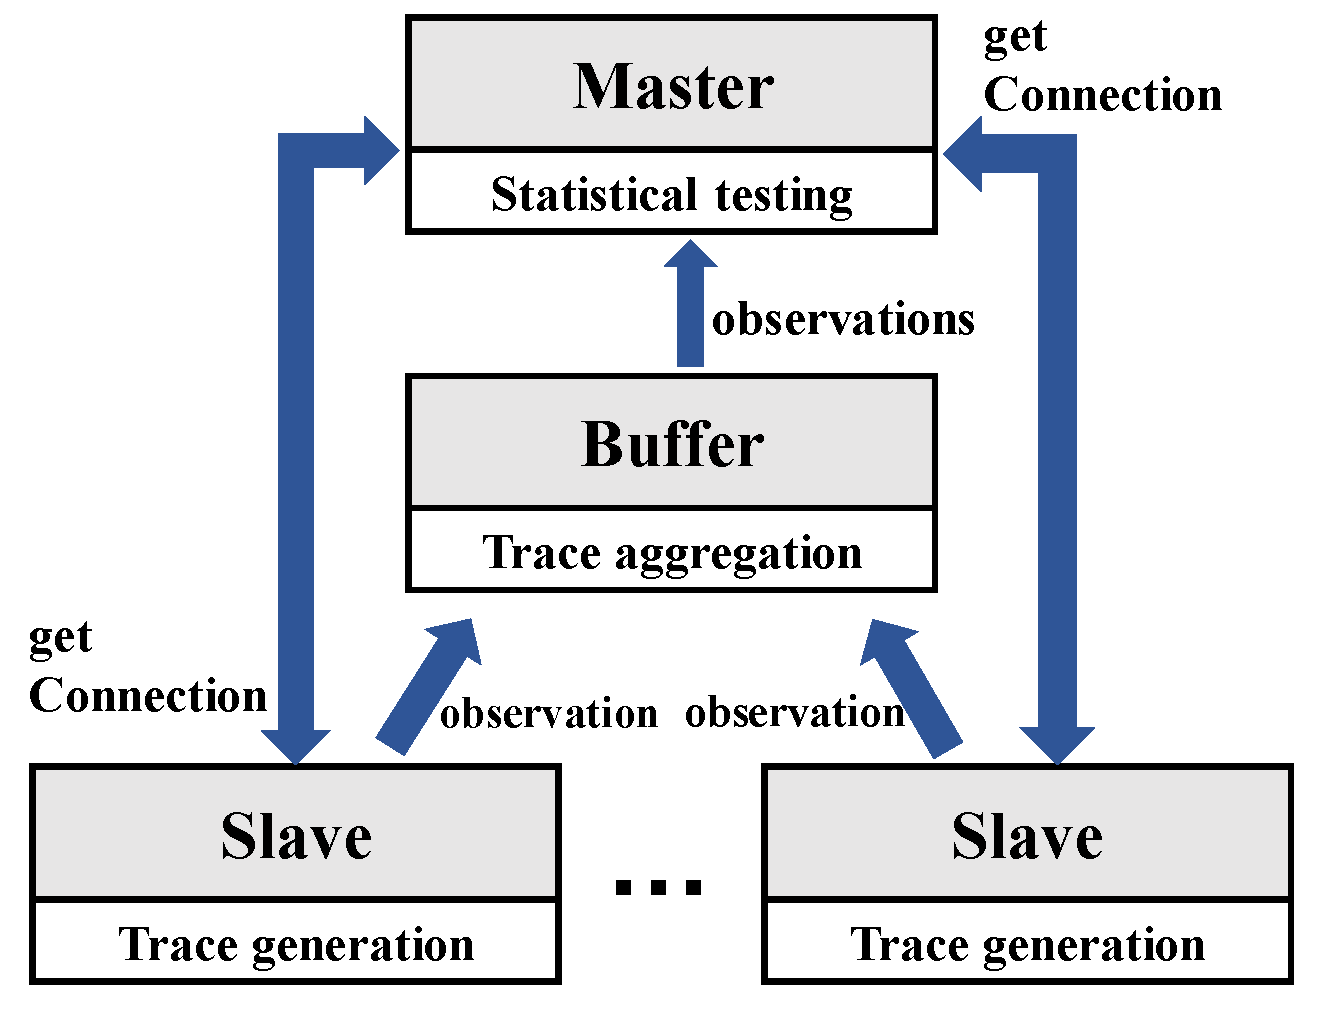
\includegraphics[width=2.5in,height=1.8in]{fig/slave-master-ach.png}
			\label{fra}}
		\hfil
		\subfigure[Communication protocol]{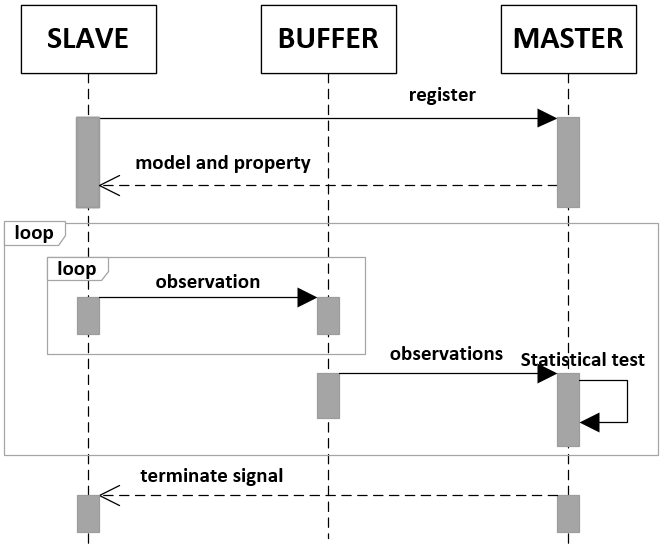
\includegraphics[width=2.5in,height=1.8in]{fig/slave-master-seq.png}
			\label{dsmc}}
	\caption{Framework of distributed SMC.}
	\label{fra_dsmc}
	}
\end{figure*}

For Unified Temporal Stochastic Logic (UTSL) model checking \cite{Younes2004Planning}, each observation involves the generation of a trajectory prefix through the discrete event simulation and the verification of a path formula over the generated trajectory prefix. Figure \ref{dsmc} illustrates the communication protocol of distributed acceptance sampling: (i)Multiple slave processes register their abilities with the master process. The master process sends the model and property to the slaves. (ii)The slave processes generate observations and send them to the buffer which is used to aggregate observations, and then the buffer send observations to the master. (iii)The master process executes statistical test. Until the statistical test terminates, it sends terminate signal to the slaves. The framework of distributed SMC is general and flexible. Based on the framework, we present our distributed BIE algorithm in the next subsection. Actually, you can adopt the framework to any other SMC algorithm, not just limits to BIE.

\subsection{Distributed bayesian interval estimation}

We can compute an interval estimate of $p=Prob(M\models\phi)$ with BIE which is a faster statistical model checking algorithm based on estimation. $\phi$ is a Probabilistic Bounded Linear Temporal Logic (PBLTL) formula \cite{baier2008principles}. $M$ is a Stochastic Hybrid Automata (SHA) model \cite{David2014Statistical}. BIE algorithm (Algorithm \ref{alg:bie}) iteratively generates trace, verifies whether it satisfies $\phi$, and then calls statistical test algorithm (Algorithm \ref{alg:sta}) to compute the estimate probability $p'$, interval ($t_0$, $t_1$) of width 2$\delta$ and posterior probability $\gamma$. Until $\gamma >= c$, the algorithm terminates and returns $t_0$, $t_1$ and $p'$, otherwise it generates another trace and repeats.
\begin{algorithm}[t]
%\SetAlgoNoLine
\KwIn{BLTL property $\phi$, half-interval size $\delta \in (0, 1/2)$, interval coverage coefficient $c \in (1/2, 1)$, Prior Beta distribution with parameters $\alpha$,$\beta$ for the (unknown) probability $p$ that the system satisfies $\phi$}
\KwOut{An interval ($t_0$, $t_1$) of width 2 $\delta$ with posterior probability at least $c$, estimate $p'$ for the true probability $p$}
$x$ = 0; $n$ = 0\;
\Repeat{$\gamma >= c$}{
        $\sigma$ = draw a simulation of the model\;
        \If{$\sigma\models\phi$\; }
        {
           $x$ = $x$ + 1\;
         }
        $n$ = $n$ + 1\;
        $t_0$,$t_1$,$p'$,$\gamma$ = \textbf{CallAlgorithm\ref{alg:sta}($\delta$, $\alpha$,$\beta$,$x$, $n$)};
      }
\caption{Bayesian estimation algorithm}
\label{alg:bie}
\end{algorithm}
\begin{algorithm}[t]
%\SetAlgoNoLine
\KwIn{half-interval size $\delta$, $\alpha$, $\beta$, positive trace number $x$, total trace number $n$}
\KwOut{An interval ($t_0$, $t_1$) of width 2$\delta$, estimate probability $p'$, posterior probability $\gamma$}
        $p'$ = (x+$\alpha$)/(n+$\alpha$+$\beta$)\;
        ($t_0$, $t_1$) = ($p^,$-$\delta$,$p^,$+$\delta$)\;
        \eIf{$t_1 > 1$ \;}
        {
           ($t_0$, $t_1$) = (1-2$\delta$,1)\;
         }{
        \If{$t_0 > 0$ \;}{
            ($t_0$, $t_1$) = (0,2$\delta$)\;
        }
          }
        $\gamma=\int_{t_0}^{t_1} {f(u|x_1,...,x_n)du}$\;
\caption{Statistical test algorithm}
\label{alg:sta}
\end{algorithm}
Based on the BIE algorithm, we implement distributed BIE algorithm with the help of our distributed SMC framework. Algorithm \ref{alg:dbeas} is the slave algorithm of distributed BIE. $B$ is the size of batch which aggregates the outcomes $x$ to reduce communication. The algorithm iteratively generates trace and verifies whether it satisfies $\phi$. Until $runs == B$, the algorithm terminates and returns the number of positive traces $sats$, otherwise it generates another trace and repeats.
\begin{algorithm}[t]
%\SetAlgoNoLine
\KwIn{BLTL property $\phi$, model $M$, batch size $B$}
\KwOut{The number of positive traces $sats$}
$sats$ = 0, $runs$ = 0\;
\Repeat{$runs$ == B}{
        $\sigma$ := getSimulationTrace($M$)\;
        \If{$\sigma \models \phi$\; }
        {
           $sats$ ++\;
         }
        $runs$ ++ \;
      }
\caption{Slave algorithm of distributed BIE}
\label{alg:dbeas}
\end{algorithm}
Algorithm \ref{alg:dbeam} is the master algorithm of distributed BIE. \emph{$K$} is the size of buffer which is used to improve concurrency since the slaves can do \emph{$K$} runs ahead of the slowest slave, and \emph{$N$} is the number of slaves. The main steps of master algorithm are as follows: (i)The slave processes register their abilities with the master. The master sends model and property to the slaves. (ii)The master algorithm chooses a slave process randomly, and then it updates batch and buffer only if the buffer size of the slave is smaller than \emph{$K$}. (iii)If the buffers of all slaves are not empty, the algorithm updates the value of \emph{$n$} and \emph{$x$}. (iv)Call algorithm \ref{alg:sta} to compute the estimate probability $p'$, interval ($t_0$, $t_1$) of width 2$\delta$ and posterior probability $\gamma$. Until $\gamma >= c$, the algorithm terminates and returns $t_0$, $t_1$ and $p'$, otherwise it repeats step (ii), (iii) and (iv).
\begin{algorithm}[t]
%\SetAlgoNoLine
\KwIn{BLTL property $\phi$, model $M$, half-interval size $\delta \in (0, 1/2)$, interval coverage coefficient $c \in (1/2, 1)$, Prior Beta distribution with parameters $\alpha$,$\beta$ for the (unknown) probability $p$ that the system satisfies $\phi$, buffer size $K$, batch size $B$, the number of nodes $N$}
\KwOut{An interval ($t_0$, $t_1$) of width 2 $\delta$ with posterior probability at least $c$, estimate $p'$ for the true probability $p$}
$x$ = 0; $n$ = 0\;
batch[0...N-1][0...K-1], buffer[0...K-1], slave[0...N-1]\;
\For{slave[i] $\in$ slave[0...N]}{
getConnection(slave[i])\;
sendModelandProperty($M$,$\phi$,slave[i])\;
}
\Repeat{$\gamma >= c$}{
        node = random(0,$N$-1)\;
        \If{$buffer[node] < K$\; }
        {
           batch[node][buffer[node]] = \textbf{CallAlgorithm\ref{alg:dbeas}(node)}\;
           buffer[node]++\;
         }
        \If{$forall(i < N) buffer[i] > 0$ \; }{
         \For{$i < N$}{
              x += batch[i][0]\;
              n += B\;
             buffer[i]--\;
              batch[i][buffer[i]] = 0\;
            }
         }
         $t_0$,$t_1$,$p'$,$\gamma$ = \textbf{CallAlgorithm\ref{alg:sta}($\delta$, $\alpha$,$\beta$ $x$, $n$)};\;
      }
\caption{Master algorithm of distributed BIE}
\label{alg:dbeam}
\end{algorithm}
\subsection{Distributed AL-SMC}
BIE algorithm has its shortcoming, because it needs more traces when it verifies the property whose probability is close to 0.5 \cite{zuliani2013bayesian}. We have proposed AL-SMC technique to solve this problem in our recent work \cite{jiangkaiqiang2016}. 
%The framework of AL-SMC is shown in Figure \ref{al-smc}. 
AL-SMC includes three main steps: (i)Sample traces are drawn from the model and input into the abstraction process to obtain abstract traces. The abstraction process includes three steps: \textbf{property-based projection, PCA-based dimension reduction \cite{dunteman1989principal} and key states extraction}. (ii)\textbf{Building and optimization of Prefix Frequency Tree (PFT)} applies the learning technique \cite{carrasco1994learning} to construct optimized PFT with abstract traces. By means of PFT, the original probability space is divided into several \textbf{sub-spaces}. (iii)\textbf{Probability evaluation via multi-BIE} invokes multiple BIE algorithms to evaluate the probabilities of sub-spaces in parallel. The detail of AL-SMC can be found in \cite{jiangkaiqiang2016}.
%\begin{figure}[htbp]
%	\centering	{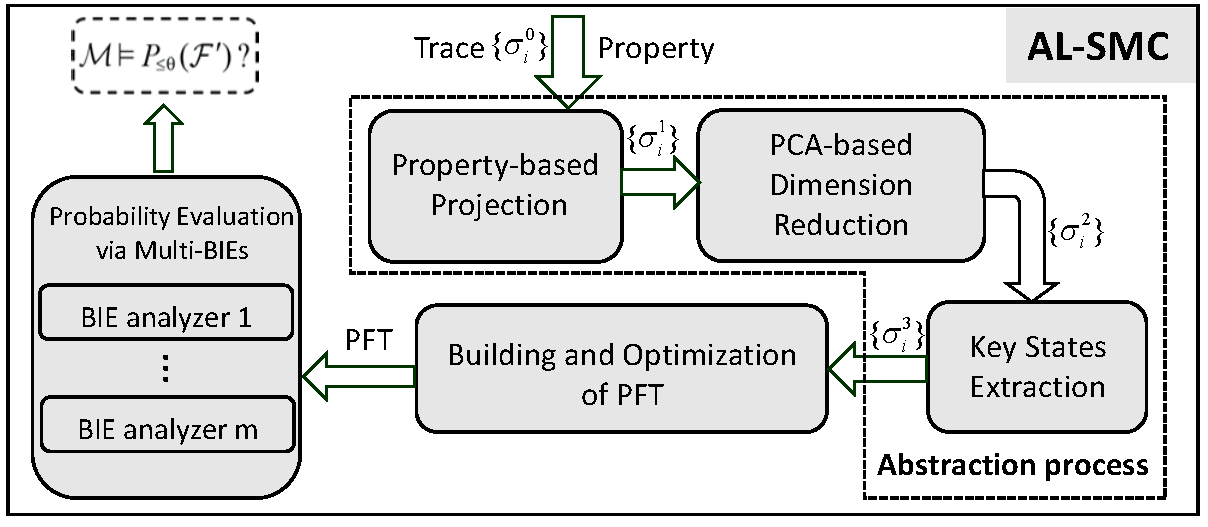
\includegraphics[width=3.2in,height=1.5in]{fig/ALSMC.png}}
%	%\vspace{0.10in}
%	\caption{The framework of AL-SMC.}\label{al-smc}
%\end{figure}

AL-SMC reduces the number of simulation traces compared with BIE algorithm, especially the verification result is close to 0.5. Therefore, the number of traces and the time consumption for generating a single trace will be effectively reduced if we apply the distributed SMC framework into AL-SMC. Fortunately, we find that AL-SMC can be  parallelized with our distributed SMC framework. Therefore, we propose DAL-SMC, whose core algorithms are shown in Algorithm \ref{alg:dalm} and Algorithm \ref{alg:dals}.

Algorithm \ref{alg:dalm} is the master algorithm of DAL-SMC, where $SN$ is the number of sample traces in abstraction process. The master algorithm contains the following steps: (i)The master process generates a set of sample traces $\sigma[0...SN-1]$ which are fed to abstraction process to obtain a set of abstract traces $\sigma'[0...SN-1]$. And then, the optimized PFT is constructed with $\sigma'[0...SN-1]$. (ii)The slave processes get connection with the master. The master process sends model, property and PFT to the slaves. (iii)The algorithm chooses a slave randomly, and then updates $batch[i][j]$ only if the buffer size of this slave is smaller than $K$. (iv)If the buffers of all slaves are not empty, the algorithm evaluates the probability and obtains $p'[j]$ and $\gamma[j]$ of each sub-space. If $\gamma[j] > c$, the evaluation of jth sub-space is terminated. (v)Until the evaluation of all sub-spaces are terminated, the algorithm estimates the probability of the whole space with $p' := \sum\limits_{i=0}^{S-1} p[i]$, otherwise it repeats step (iii), (iv) and (v).
\begin{algorithm}[t]
%\SetAlgoNoLine
\KwIn{BLTL property $\phi$, model $M$, half-interval size $\delta \in (0, 1/2)$, interval coverage coefficient $c \in (1/2, 1)$, Prior Beta distribution with parameters $\alpha$, $\beta$ for the (unknown) probability $p$ that the system satisfies $\phi$, buffer size $K$, batch size $B$, the number of nodes $N$, the number of sample traces $SN$ }
\KwOut{Prefix frequency tree $T$, estimate $p'$ for the true probability $p$}
$\sigma[0...SN-1]$ = getSampleTraces($M$)\;
$\sigma'[0...SN-1]$ = abstractTraces($\sigma[0...SN-1]$)\;
$T$ = ConstructPFT($\sigma'[0...SN-1]$)\;
$d$ = getSubSpacesNum($T$)\;
\For{slave[i] $\in$ slave[0...N]}{
getConnection(slave[i])\;
sendModelandPropertyandPFT($M$,$\phi$,$T$,slave[i])\;
}
x[0...d-1], n\;
batch[0...N-1][0...K-1][0...d-1], buffer[0...K-1], slave[0...N-1]\;
\Repeat{forall(ter[i] $\in$ ter[0...d-1])==true}{
        node = random(0,$N$-1)\;
        \If{$buffer[node] < K$ \; }
        {
           batch[node][buffer[node]][0...d-1] = \textbf{CallAlgorithm\ref{alg:dals}(node)}\;
           buffer[node]++\;
         }
        \If{$forall(i < N) buffer[i] > 0$ \; }{
         \For{$i < N$}{
              x[0...d-1] += batch[i][0][0...d-1]\;
              n += B\;
              buffer[i]--\;
              batch[i][buffer[i]] = $\Phi$\;
            }
         }
         ter[0...d-1] = false\;
         j = findUnTerminateBIE(ter[0...d-1])\;
         $p'[j]$,$\gamma[j]$ = \textbf{CallAlgorithm\ref{alg:sta}($\delta$, $\alpha$,$\beta$ $x[j]$, $n$)};\;
        \If{$\gamma[j] > c$\; }
        {
           $ter[j] = true$ \;
         }
      }
 $p' = \sum\limits_{i=0}^{d-1} p'[i]$\;
\caption{Master algorithm of DAL-SMC}
\label{alg:dalm}
\end{algorithm}
Algorithm \ref{alg:dals} is the slave algorithm of DAL-SMC. $T$ is the optimized PFT which is constructed in master algorithm. $d$ is the number of leaf nodes in optimized PFT tree, i.e., the number of sub-spaces. $sats[i]$ is the number of satisfying traces in ith sub-space. The slave process iteratively generates trace $\sigma$ which is the input of abstraction process to obtain the abstract trace $\sigma'$. If $\sigma'$ satisfies $\phi$, the algorithm finds a sub-space with $\sigma'$ and $T$. Until $runs == B$, the algorithm terminates and returns $sats[0...S-1]$, otherwise, it generates another trace and repeats.
\begin{algorithm}[t]
%\SetAlgoNoLine
\KwIn{BLTL property $\phi$, model $M$, batch size $B$, prefix frequency tree $T$, the number of sub-spaces $d$}
\KwOut{The number of positive traces in sub-spaces $sats[0...d-1]$}
$sats[0...d-1]$, $runs$ = 0\;
\Repeat{$runs$ == B}{
        $\sigma$ = getSimulationTrace($M$)\;
        $\sigma'$ = abstractTrace($\sigma$)\;
        \If{$\sigma \models \phi$\; }
        {
           i = findSubSpace($\sigma'$, $T$)\;
           $sats[i]$ ++\;
         }
        $runs$ ++ \;
      }
\caption{Salve algorithm of DAL-SMC}
\label{alg:dals}
\end{algorithm}
DAL-SMC is more efficient than distributed BIE with the help of abstraction and learning techniques, and the advantages of DAL-SMC are obvious. Firstly, the slave process of DAL-SMC generates less traces, particularly in verifying the property whose probability is close to 0.5. Secondly, the master of DAL-SMC evaluates the probability with multiple BIEs, thus the statistic process is faster than that of distributed BIE algorithm. However, DAL-SMC has bigger statistical error due to the usage of multi-BIE in statistic process. In the remainder of the paper, we focus on the performance analysis of DAL-SMC.  In the next subsection, we will introduce our parameter optimization method to reduce the statistical error of DAL-SMC. 
\subsection{Parameter optimization of DAL-SMC}
In order to reduce the statistical error of DAL-SMC, we introduce two parameter optimization methods: \textbf{$r$ optimization} is used to divide the probability space more evenly, and \textbf{$\delta$ prediction} is used to predict half-interval size of the BIE algorithm used in each sub-space.

\textbf{$r$ optimization}: For DAL-SMC, we divide the probability space into several sub-spaces by building and optimizing the PFT. Note that the number of sub-spaces is determined by the leaf nodes of optimized PFT. Therefore, we need input the reduction degree $r$ of PFT into the optimization algorithm to generate optimized PFT. However, the value of $r$ is difficult to predict. On one hand, if the value of $r$ is too large, we will obtain a large number of sub-spaces and the error of the algorithm will be enlarged. On the other hand, if the value of $r$ is too small, we will obtain few sub-spaces and the efficiency of the algorithm will be reduced. To solve the problem, we obtain the optimized value of $r$ with genetic algorithm \cite{DBLP:books/daglib/0019871}. 
\begin{equation}
\centering
\label{formula1}
r_k = M - \sum\limits_{i=1}^k \sum\limits_{j=1}^k |T_i - T_j| 
\end{equation}
Suppose $k$ is the population quantity in genetic algorithm, i.e., the number of sub-spaces of each generation. $T_i$ is the number of satisfying traces in $ith$ sub-space. In order to obtain the optimal $r$, we need to divide the probability space more evenly and ensure a moderate number of sub-spaces. Therefore, we adopt formula \ref{formula1} as evaluation function and $k \geq 6 \&\& k \leq 10$ as constraint function of genetic algorithm. $M$ is a large positive number, if we divide the probability space more evenly, the value of $\sum\limits_{i=1}^k \sum\limits_{j=1}^k |T_i - T_j|$ is smaller. Thus, we obtain the optimal $r$ which helps to get the maximum $M$. 

\textbf{$\delta$ prediction}:
Through building and optimizing of PFT, we obtain several sub-spaces. Then we execute BIE algorithm for each sub-space, each BIE algorithm has its half-interval size and interval coverage coefficient. In algorithm \ref{alg:dals}, we suppose all BIE algorithms have the same $\delta$ and $c$. However, the probabilities of some sub-spaces may have a big difference. For instance, we suppose the half-interval sizes of all BIE algorithms are 0.1, but there may be a sub-space whose probability is less than 0.1, thus the half-interval size of this BIE algorithm is unreasonable. It will lead to a large statistical error. To solve this problem, we use the leaf nodes of PFT to predict the half-interval size of $mth$ BIE algorithm as shown in formula \ref{formula2}. Note that $k$ is the number of sub-spaces, $T_m$ is the number of satisfying traces in $m$-$th$ sub-space, and $N_i$ is the number of total traces in $i$-$th$ sub-space. $\eta$ is half-interval rate, the $\eta$ is bigger, the probability is more precise. By means of formula \ref{formula2}, the half-interval size of each BIE is more accurate.
\begin{equation}
\label{formula2}
\delta_m = T_m / \sum\limits_{i=1}^k N_i / \eta
\end{equation}
